	\section{Unidad 2}
	    \subsection{Números decimales}

      \subsubsection{Ubicación en la recta numérica}

      \questionboxed[4]{Escribe el número que representa el punto indicado en la recta numérica de cada uno de los siguientes incisos.

            \begin{multicols}{3}
                  \begin{parts}
                        \part 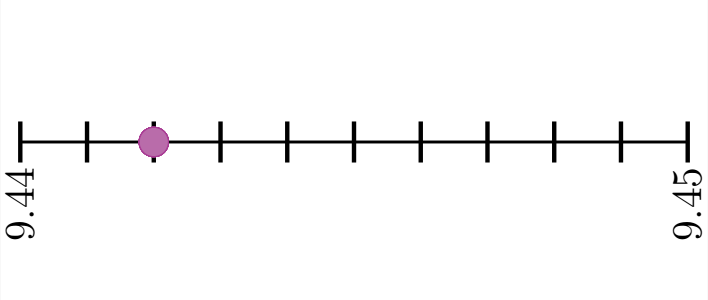
\includegraphics[width=\linewidth]{../images/recta_num_9.442.png}\\[-0.5em]  \fillin[$9.44$][1.5in]
                        \part 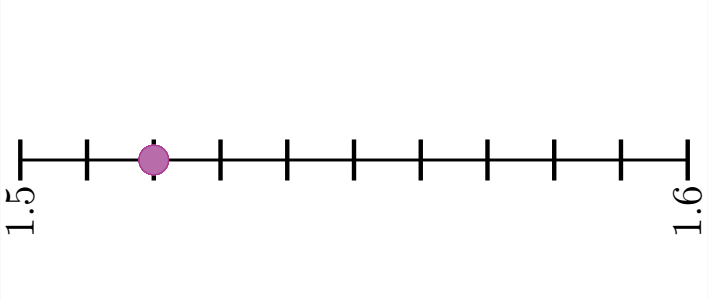
\includegraphics[width=\linewidth]{../images/recta_num_1.52.png} \\[-0.5em] \fillin[$1.52$][1.5in]
                        % \part 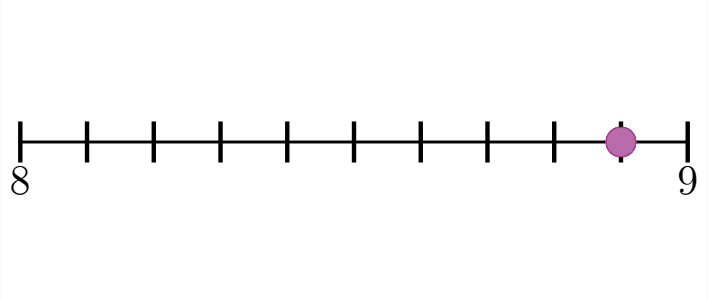
\includegraphics[width=\linewidth]{../images/recta_num_8.9.png}  \\[-0.5em]  \fillin[$8.9$][1.5in]
                        \part 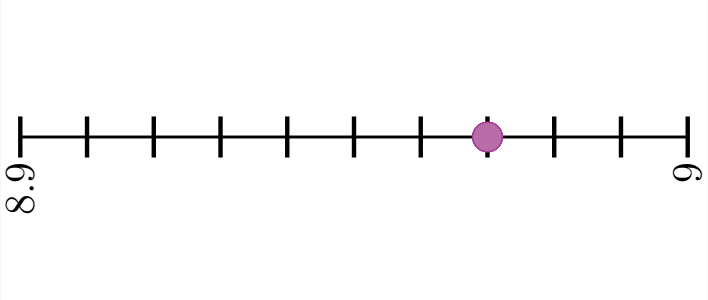
\includegraphics[width=\linewidth]{../images/recta_num_8.97.png} \\[-0.5em]  \fillin[$8.97$][1.5in]
                        \part 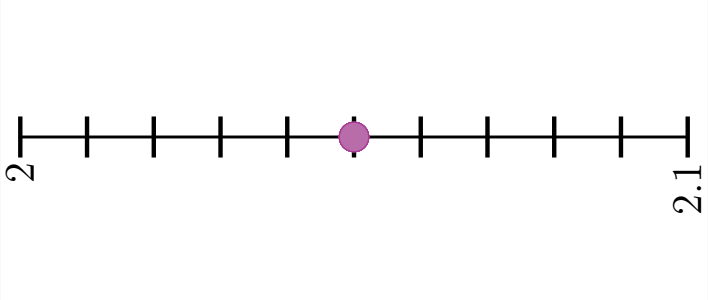
\includegraphics[width=\linewidth]{../images/recta_num_2.05.png} \\[-0.5em]  \fillin[$2.05$][1.5in]
                        \part 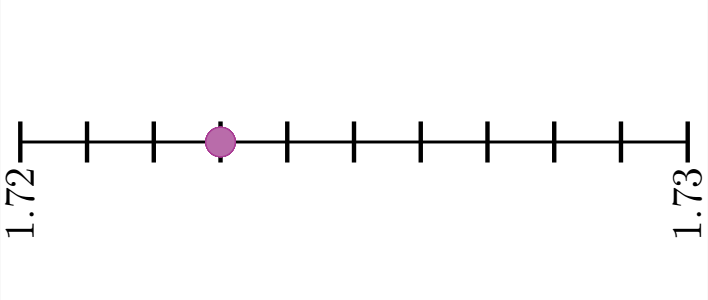
\includegraphics[width=\linewidth]{../images/recta_num_1.723.png}\\[-0.5em]  \fillin[$1.723$][1.5in] \\[-1.5em]
                        \part 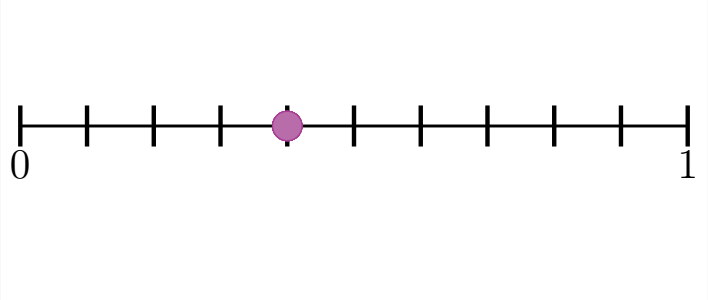
\includegraphics[width=\linewidth]{../images/recta_num_0.4.png}  \\[-0.5em]  \fillin[$0.4$][1.5in] \\[-1.5em]
                        \part 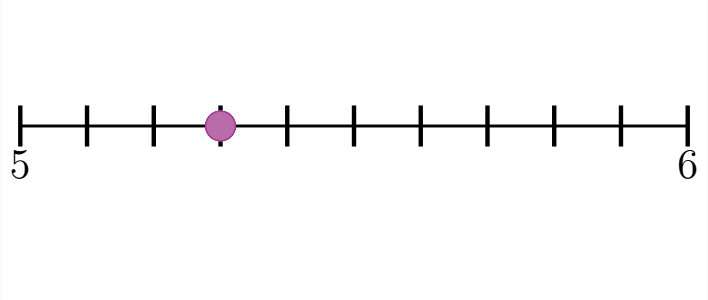
\includegraphics[width=\linewidth]{../images/recta_num_5.3.png}  \\[-0.5em]  \fillin[$5.3$][1.5in] \\[-1.5em]
                        \part 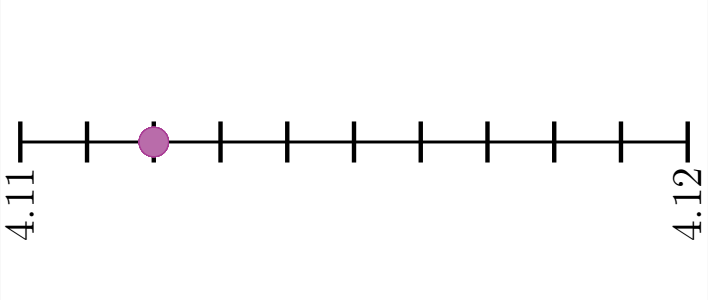
\includegraphics[width=\linewidth]{../images/recta_num_4.112.png}\\[-0.5em]  \fillin[$4.112$][1.5in] \\[-1.5em]
                        \part 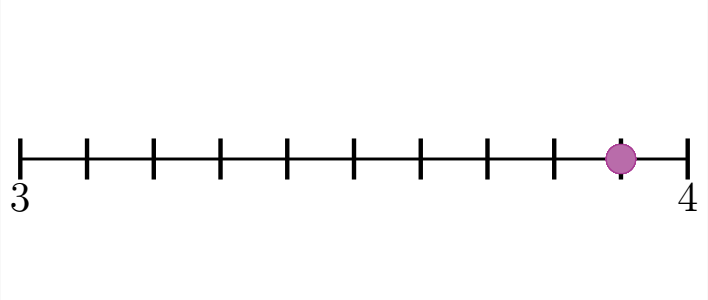
\includegraphics[width=\linewidth]{../images/recta_num_3.9.png} \\[-0.5em]  \fillin[$3.9$][1.5in]
                  \end{parts}
            \end{multicols}
      }

      \subsubsection{Porcentajes a decimal}
     
      \questionboxed[4]{Escribe el número decimal que representa cada porcentaje:

            \begin{multicols}{3}
                  \begin{parts}
                        \part Convierte 50\% a  decimal. \fillin[$0.5$][0in]
                        \part Convierte 25\% a  decimal. \fillin[$0.25$][0in]
                        \part Convierte 12\% a  decimal. \fillin[$0.12$][0in]
                        \part Convierte 22.9\% a  decimal. \fillin[$0.229$][0in]
                        \part Convierte 6.2\% a  decimal. \fillin[$0.062$][0in]
                        \part Convierte 0.5\% a  decimal. \fillin[$0.005$][0in]
                  \end{parts}
            \end{multicols}
      }

      \subsubsection{Operaciones con múltiplos de 10}
 
      \questionboxed[4]{Realiza las siguientes operaciones con múltiplos de 10:

            \begin{multicols}{3}
                  \begin{parts}
                        \part $56.9 \times 100=$ \fillin[$5690$][0in]
                        \part $0.712 \times 1000=$ \fillin[$712$][0in]
                        \part $0.204 \times 10=$ \fillin[$2.04$][0in]
                        \part $70 \times 100=$ \fillin[$7000$][0in]
                        \part $0.5 \times 1000=$ \fillin[$500$][0in]
                        \part $0.25 \times 10=$ \fillin[$2.5$][0in]
                  \end{parts}
            \end{multicols}
      }

      \subsubsection{Conversión de fracciones a decimales}
  
      \questionboxed[4]{Convierte las siguientes fracciones a decimales:
          
      \begin{multicols}{3}
                  \begin{parts}
                        \part $\dfrac{7}{20}=$ \fillin[$0.35$][0in]
                        \part $\dfrac{3}{4}=$ \fillin[$0.75$][0in]
                        \part $\dfrac{50}{2}=$ \fillin[$25$][0in]
                        % \part $\dfrac{1}{4}=$ \fillin[$0.25$][0in]
                        \part $\dfrac{1}{8}=$ \fillin[$0.125$][0in]
                        \part $\dfrac{5}{4}=$         \fillin[$1.25$][0in] 
                        \part $\dfrac{7}{20}=$        \fillin[$0.35$][0in] 
                        \part $\dfrac{1927}{1000}=$   \fillin[$1.927$][0in]
                        \part $\dfrac{9}{4}=$         \fillin[$2.25$][0in] 
                        \part $\dfrac{3}{20}=$        \fillin[$0.15$][0in] 
                        \part $\dfrac{13}{100}=$      \fillin[$0.13$][0in]                         
                        \part $\dfrac{11}{50}=$       \fillin[$0.22$][0in] 
                        % \part $\dfrac{459}{100}=$    \fillin[$4.59$][0in] 
                        \part $\dfrac{19}{25}=$       \fillin[$0.76$][0in] 
                        % \part $\dfrac{2039}{1000}=$   \fillin[$2.039$][0in]
                  \end{parts}
            \end{multicols}
      }

      \subsubsection{Conversión de decimales a fracciones}
   
      \questionboxed[4]{Convierte los siguientes números decimales a una fracción simplificada a su mínima expresión:
           
      \begin{multicols}{2}
                  \begin{parts}
                        \part $0.04=$ \fillin[$\dfrac{1}{25}$][0in]
                        \part $0.19=$ \fillin[$\dfrac{19}{100}$][0in]
                        \part $0.25=$ \fillin[$\dfrac{1}{4}$][0in]
                        \part $0.5=$ \fillin[$\dfrac{1}{2}$][0in]
                        \part $0.75=$ \fillin[$\dfrac{3}{4}$][0in]
                        \part $0.125=$ \fillin[$\dfrac{1}{8}$][0in]
                        \part $0.875=$       \fillin[$\dfrac{7}{8}$][0in] 
                        \part $0.45=$    \fillin[$\dfrac{9}{20}$][0in]    
                        \part $0.002=$      \fillin[$\dfrac{1}{500}$][0in]
                        \part $0.9=$       \fillin[$\dfrac{9}{10}$][0in]  
                  \end{parts}
            \end{multicols}
      }

    \subsection{Operaciones con decimales}
	\subsubsection{Suma de decimales}
	\questionboxed[5]{ Realiza las siguientes sumas de decimales:

		\begin{multicols}{5}
			\begin{parts}
				\part 
				\ifprintanswers{\opadd[hfactor=decimal,resultstyle=\color{red},carryadd=true]{16.981}{15.891}}
				\else{\opadd[hfactor=decimal,resultstyle=\color{white},displayintermediary=None,carryadd=false,carrysub=false]{16.981}{15.891}}\fi				
				\part 
				\ifprintanswers{\opadd[hfactor=decimal,resultstyle=\color{red},carryadd=true]{620.64}{515.92}}
				\else{\opadd[hfactor=decimal,resultstyle=\color{white},displayintermediary=None,carryadd=false,carrysub=false]{620.64}{515.92}}\fi
				\part 
				\ifprintanswers{\opadd[hfactor=decimal,resultstyle=\color{red},carryadd=true]{24.97}{19.34}}
				\else{\opadd[hfactor=decimal,resultstyle=\color{white},displayintermediary=None,carryadd=false,carrysub=false]{24.97}{19.34}}\fi
				\part 
				\ifprintanswers{\opadd[hfactor=decimal,resultstyle=\color{red},carryadd=true]{509.44}{338.79}}
				\else{\opadd[hfactor=decimal,resultstyle=\color{white},displayintermediary=None,carryadd=false,carrysub=false]{509.44}{338.79}}\fi
				\part 
				\ifprintanswers{\opadd[hfactor=decimal,resultstyle=\color{red},carryadd=true]{33.31}{19.54}}
				\else{\opadd[hfactor=decimal,resultstyle=\color{white},displayintermediary=None,carryadd=false,carrysub=false]{33.31}{19.54}}\fi
			\end{parts}
		\end{multicols}
	}

	\subsubsection{Resta de decimales}

	\questionboxed[5]{ Realiza las siguientes restas de decimales:

		\begin{multicols}{3}
			\begin{parts}\large
				\part \ifprintanswers{   \opsub[hfactor=decimal,resultstyle=\color{red},carryadd=true,carrysub=true]{55.394}{49.093} }
				\else{            \opsub[hfactor=decimal,resultstyle=\color{white},carryadd=false,carrysub=false]{55.394}{49.093}\\[0.5cm] }
				\fi

				\part \ifprintanswers{   \opsub[hfactor=decimal,resultstyle=\color{red},carryadd=true,carrysub=true]{55.394}{49.093} }
				\else{            \opsub[hfactor=decimal,resultstyle=\color{white},carryadd=false,carrysub=false]{55.394}{49.093}\\[0.5cm] }
				\fi

				\part \ifprintanswers{   \opsub[hfactor=decimal,resultstyle=\color{red},carryadd=true,carrysub=true]{55.394}{49.093} }
				\else{            \opsub[hfactor=decimal,resultstyle=\color{white},carryadd=false,carrysub=false]{55.394}{49.093}\\[0.5cm] }
				\fi

				\part \opsub[hfactor=decimal,resultstyle=\color{white},displayintermediary=None,carryadd=false,carrysub=false]{5.134}{2.347}\\[1em]
				\part \opsub[hfactor=decimal,resultstyle=\color{white},displayintermediary=None,carryadd=false,carrysub=false]{968.31}{134.67}\\[1em]
			\end{parts}
		\end{multicols}

	}

	\subsubsection{Multiplicación de decimales}

	\questionboxed[5]{ Realiza las siguientes multiplicaciones de decimales:

		\begin{multicols}{3}
			\begin{parts}
				\part \opmul[hfactor=decimal,resultstyle=\color{white},displayintermediary=None]{17.31}{4.81}\\[1em]
				\part \opmul[hfactor=decimal,resultstyle=\color{white},displayintermediary=None]{12.34}{7.21}\\[1em]
				\part \opmul[hfactor=decimal,resultstyle=\color{white},displayintermediary=None]{198.4}{12.2}\\[1em]
			\end{parts}
		\end{multicols}

	}

	\subsubsection{División de decimales}

	\questionboxed[5]{ Realiza las siguientes divisiones con decimales:

		\begin{multicols}{3}
			\begin{parts}\large
				\part ${12.4}\divisionsymbol{5.1}=$\\[1em]
				\part ${8.32}\divisionsymbol{1.2}=$\\[1em]
				\part ${54}\divisionsymbol{2.5}=$\\[1em]
			\end{parts}
		\end{multicols}

	}

	\subsubsection{Resolución de problemas}

	\questionboxed[5]{Resuelve los siguientes problemas:

		\begin{parts}
			\part Una pintura tiene un costo de 33.24 pesos el litro, una persona compra 53 litros. ¿Cuánto debe pagar?

			\begin{solutionbox}{2cm}
				\opmul[hfactor=decimal,resultstyle=\color{white},displayintermediary=None,carryadd=false,carrysub=false]{33.24}{53}
			\end{solutionbox}

			\part La mamá de Susana compró 11 metros de franela y pagó 103.40 pesos. ¿Cuánto cuesta el metro de franela?

			\begin{solutionbox}{2cm}
				\opdiv[hfactor=decimal,resultstyle=\color{white},displayintermediary=None,carryadd=false,carrysub=false]{103.40}{11}
			\end{solutionbox}

			\part El precio de 385 artículos comerciales es de 1,232 pesos. ¿Cuál es el precio unitario de cada artículo?

			\begin{solutionbox}{2cm}
				\opdiv[hfactor=decimal,resultstyle=\color{white},displayintermediary=None,carryadd=false,carrysub=false]{1232}{385}
			\end{solutionbox}
		\end{parts}
	}


	\newpage
	\subsection{Porcentajes}
	\subsubsection{Porcentajes a decimal}
	\questionboxed[5]{ Escribe como decimal los siguientes porcentajes:
		\begin{multicols}{3}
			\begin{parts}
				\part 25\% = \fillin[0.25][0in]
				\part 75\% = \fillin[0.75][0in]
				\part 50\% = \fillin[0.5][0in]
				\part 10\% = \fillin[0.1][0in]
				\part 5\% = \fillin[0.5][0in]
				\part 0.5\% = \fillin[0.1][0in]
			\end{parts}
		\end{multicols}
	}

	\subsubsection{Decimal a porcentaje}
	\questionboxed[5]{ Escribe como porcentaje los siguientes decimales:
		\begin{multicols}{3}
			\begin{parts}
				\part $0.52$  = \fillin[52\%][0in]
				\part $0.09$  = \fillin[9\%][0in]
				\part $6.5$   = \fillin[650\%][0in]
				\part $0.704$ = \fillin[70.4\%][0in]
				\part $0.1$   = \fillin[10\%][0in]
				\part $1$     = \fillin[100\%][0in]
			\end{parts}
		\end{multicols}
	}

	\subsubsection{Porcentaje de cantidades}
	\questionboxed[5]{ Calcula el porcentaje de las siguientes cantidades:
		\begin{multicols}{3}
			\begin{parts}
				\part 80\% de 250 = \fillin[200][0.5in]
				\part 15\% de 900 = \fillin[135][0.5in]
				\part 50\% de 600 = \fillin[300][0.5in]
				\part 13\% de 1200 = \fillin[156][0.5in]
				\part 5\% de 715 = \fillin[35.75][0.5in]
				\part 35\% de 415 = \fillin[145.25][0.5in]

				\part Si se sabe que 210 es el 21\% de cierta cantidad, ¿cuál es esta cantidad?
				\begin{solutionbox}{3cm}
					Para conocer la cantidad, se debe dividir 210 entre 21; entonces:
					\[100\times\dfrac{210}{21}=10\]
				\end{solutionbox}

				\part Si se sabe que 200 es el 250\% de cierta cantidad, ¿cuál es esta cantidad?
				\begin{solutionbox}{3cm}
					Para conocer la cantidad, se debe dividir 200 entre 250; entonces:
					\[100\times\dfrac{200}{250}=80\]
				\end{solutionbox}

				\part Si se sabe que 120 es el 35\% de cierta cantidad, ¿cuál es esta cantidad?
				\begin{solutionbox}{3cm}
					Para conocer la cantidad, se debe dividir 120 entre 35; entonces:
					\[100\times\dfrac{120}{35}=342.86\]
				\end{solutionbox}
			\end{parts}
		\end{multicols}
	}

	% \questionboxed[5]{Resuelve los siguientes problemas con porcentajes:
	%       \begin{parts}

	%       \end{parts}
	% }

	\subsubsection{Resolución de problemas}
	\questionboxed[5]{ Resuelve los siguientes problemas:
		\begin{parts}
			\part El costo de una computadora es de 12220 pesos, si la tasa de impuesto es del 15\%. ¿Cuánto será el total a pagar por la computadora?
			\begin{solutionbox}{2.5cm}
				Para conocer el total a pagar por la computadora, se debe multiplicar 12220 por 15\%; entonces:
				\[12220\times 115\%= 14053\]
				Por lo tanto, el total a pagar por la computadora es de 14053 pesos.
			\end{solutionbox}

			\part El 24\% de los habitantes de un pueblo tienen menos de 30 años. ¿Cuántos habitantes tiene el pueblo si hay 120 jóvenes menores de 30 años?
			\begin{solutionbox}{2.5cm}
				Para conocer el total de habitantes del pueblo, se debe dividir 120 entre 24\%; entonces:
				\[100\times\dfrac{120}{24}=500\]
				Por lo tanto, el pueblo tiene 500 habitantes.
			\end{solutionbox}
		\end{parts}
	}

	\subsection{Potencias y raíces}
	\subsubsection{Potenciación}
	\questionboxed[5]{ Realiza las siguientes potencias:
		\begin{multicols}{3}
			\begin{parts}
				\part $2^3=$ \fillin[8][0in]
				\part $3^2=$ \fillin[9][0in]
				\part $5^2=$ \fillin[25][0in]
				\part $10^4=$ \fillin[10000][0in]
				\part $3^5=$ \fillin[243][0in]
				\part $\left(\dfrac{1}{3}\right)^3=$ \fillin[$\dfrac{1}{27}$][0in]
				\part $\left(\dfrac{2}{3}\right)^4=$ \fillin[$\dfrac{16}{81}$][0in]
				\part $\left(\dfrac{1}{9}\right)^2=$ \fillin[$\dfrac{1}{81}$][0in]
				\part $\left(\dfrac{4}{3}\right)^2=$ \fillin[$\dfrac{1}{1000}$][0in]
				\part $\left(\dfrac{3}{2}\right)^5=$ \fillin[$\dfrac{1}{8}$][0in]
			\end{parts}
		\end{multicols}
	}

	\subsubsection{Notación científica}
	\questionboxed[5]{Escribe la forma desarrollada de los siguientes números:
		\begin{multicols}{3}
			\begin{parts}
				\part $1.0934\times10^{4}=$
				\part $3.39\times10^{3}=$
				\part $12\times10^{5}=$
				\part $4\times10^{2}=$
				\part $2.08\times10^{6}=$
				\part $0.5\times10^{3}=$
			\end{parts}
		\end{multicols}
	}

	\questionboxed[5]{Escribe con notación científica los siguientes números:
		\begin{multicols}{3}
			\begin{parts}
				\part $7600=$
				\part $0.04=$
				\part $5000000=$
				\part $0.1=$
				\part $25=$
				\part $1.01=$
			\end{parts}
		\end{multicols}
	}


	\subsubsection{Raíces}
	\questionboxed[5]{Calcula las siguientes raíces cuadradas:
		\begin{multicols}{3}
			\begin{parts}
				\part $\sqrt{169}=$
				\part $\sqrt{1.44}=$
				\part $\sqrt{0.09}=$
				\part $\sqrt{2.25}=$
				\part $\sqrt{196}=$
				\part $\sqrt{900}$
			\end{parts}
		\end{multicols}
	}

	\subsection{Sistema de unidades}
	\subsubsection{Unidades de longitud y masa}
	\questionboxed[5]{Convierte las siguientes unidades de longitud y de masa como se te pide:
		\begin{parts}
			\part Convierte 4.9 kilómetros a metros.
			\part Convierte 34 metros a hectómetros
			\part Convierte 98 milímetros a centímetros
			\part Convierte 134 kilómetros a metros
			\part Convierte 134 centímetros a decámetros
			\part Convierte 342 gramos a hectogramos.
			\part Convierte 8334 centigramos a gramos.
			\part Convierte 93.4 miligramos a centigramos.
			\part Convierte 29 decagramos a miligramos.
			\part Convierte 9 gramos a miligramos.
		\end{parts}
	}

	\subsubsection{Unidades de capacidad}
	\questionboxed[5]{Convierte las siguientes unidades de capacidad como se te pide:
		\begin{parts}
			\part Convierte 27 hectolitros a decilitros.
			\part Convierte 8 mililitros a centilitros.
			\part Convierte 1094 mililitros a decilitros.
			\part Convierte 702 mililitros a decilitros.
			\part Convierte 19 litros a mililitros.
			\part Convierte 8200 litros a metros cúbicos.
			\part Convierte 4.8 decímetros cúbicos a litros.
			\part Convierte 750 litros a metros cúbicos.
			\part Convierte 567 milímetros cúbicos a litros.
			\part Convierte 4100 litros a metros cúbicos.

		\end{parts}
	}
	\subsubsection{Unidades de área y volumen}
	\questionboxed[5]{Convierte las siguientes unidades de área y volumen como se te pide:
		\begin{parts}
			\part Convierte 8.03 metros cúbicos a milímetros cúbicos
			\part Convierte 8 kilómetros cuadrados a metros cuadrados
			\part Convierte 88 metros cuadrados a kilómetros cuadrados
			\part Convierte 18 decámetros cúbicos a milímetros cúbicos
			\part Convierte 801 milímetros cuadrados a decámetros cuadrados
		\end{parts}
	}